% Poster, CoRL 2026 Workshop "Do Robots Need World Models?" (A0 portrait). Numbers match main.tex.
\documentclass[25pt, a0paper, portrait, margin=0mm, innermargin=18mm, blockverticalspace=14mm,
  colspace=16mm, subcolspace=0mm]{tikzposter}
\usepackage{booktabs,graphicx,amsmath,qrcode}
\usepackage[scaled]{helvet}
\renewcommand{\familydefault}{\sfdefault}

\definecolor{ink}{HTML}{1B2430}
\definecolor{accent}{HTML}{1F5FAD}
\definecolor{warm}{HTML}{C0392B}
\definecolor{paper}{HTML}{FFFFFF}
\definecolor{soft}{HTML}{EEF3FA}
\definecolorstyle{clean}{}{
  \colorlet{backgroundcolor}{paper}
  \colorlet{framecolor}{paper}
  \colorlet{titlefgcolor}{white}
  \colorlet{titlebgcolor}{accent}
  \colorlet{blocktitlebgcolor}{paper}
  \colorlet{blocktitlefgcolor}{accent}
  \colorlet{blockbodybgcolor}{paper}
  \colorlet{blockbodyfgcolor}{ink}
  \colorlet{innerblocktitlebgcolor}{soft}
  \colorlet{innerblocktitlefgcolor}{ink}
  \colorlet{innerblockbodybgcolor}{soft}
  \colorlet{innerblockbodyfgcolor}{ink}
  \colorlet{notefgcolor}{ink}
  \colorlet{notebgcolor}{soft}
  \colorlet{notefrcolor}{soft}
}
\usecolorstyle{clean}
\usebackgroundstyle{Empty}
\usetitlestyle{Filled}
\useblockstyle[titleleft, titleinnersep=6mm, bodyinnersep=8mm, linewidth=0pt]{Basic}
\useinnerblockstyle[roundedcorners=8, linewidth=0pt]{Default}
\settitle{%
  \begin{minipage}[c]{0.80\linewidth}\raggedright\color{white}
    {\fontsize{78}{92}\selectfont\bfseries Pixels Without Geometry?}\\[6mm]
    {\fontsize{46}{56}\selectfont Auditing the 3D Consistency of Video World Models with Structure-from-Motion}\\[14mm]
    {\fontsize{36}{44}\selectfont Hamza Naeem \;\textbullet\; Northeastern University \;\textbullet\; naeem.ha@northeastern.edu}\\[4mm]
    {\fontsize{28}{34}\selectfont CoRL 2026 Workshop: Do Robots Need World Models? \;\textbullet\; Austin, TX}
  \end{minipage}\hfill
  \begin{minipage}[c]{0.15\linewidth}\centering\color{white}
    \colorbox{white}{\color{black}\qrcode[height=6cm]{https://github.com/naeem-ha/wm-geometry}}\\[3mm]
    {\fontsize{22}{26}\selectfont code}
  \end{minipage}}
\title{}\author{}\institute{}

\newcommand{\lead}[1]{{\fontsize{44}{56}\selectfont #1}}
\newcommand{\hl}[1]{{\color{warm}\bfseries #1}}

\begin{document}
\maketitle[width=\paperwidth, linewidth=0pt, innersep=30mm, titletotopverticalspace=0mm, titletoblockverticalspace=16mm]

\block[bodyoffsety=0mm]{}{
  \innerblock{}{
    \centering\lead{\textbf{A frozen first frame beats real robot footage on standard geometric
    consistency scores.}\\[4mm] Raw scores reward predictions that barely move. Compare each prediction
    against \hl{real footage with the same image motion} before reading anything into it.}
  }
}

\begin{columns}
\column{0.5}
\block{Question}{
  Can a video model's predicted future of the robot's wrist camera be read as one rigid scene seen
  by a moving camera? SfM and feed-forward reconstruction are increasingly used to answer this, but
  a static camera gives clean matches, blur removes features without changing geometry, and
  non-rigid distortion can still register.
}

\block{Setup}{
  \begin{itemize}
    \item \textbf{Data:} 60 DROID-100 wrist-camera clips, 5\,s, highest image motion per episode
    \item \textbf{Models:} LTX-Video, CogVideoX-5B, Wan2.2-5B (first frame + instruction);
      Ctrl-World (action-conditioned, recorded end-effector poses)
    \item \textbf{Scores:} COLMAP registration, SIFT+MAGSAC++ match failure, inliers, Sampson error,
      VGGT depth disagreement, camera-path error
    \item \textbf{Controls (real footage):} non-rigid warps 1--8\,px, sharpness-matched blur, slowed,
      unrelated frames, frozen frame, and per-clip \hl{motion-matched} same-episode footage
    \item Paired bootstrap 95\% CIs; 25 clips shared by all models
  \end{itemize}
}

\block{What the predictions look like}{
  \centering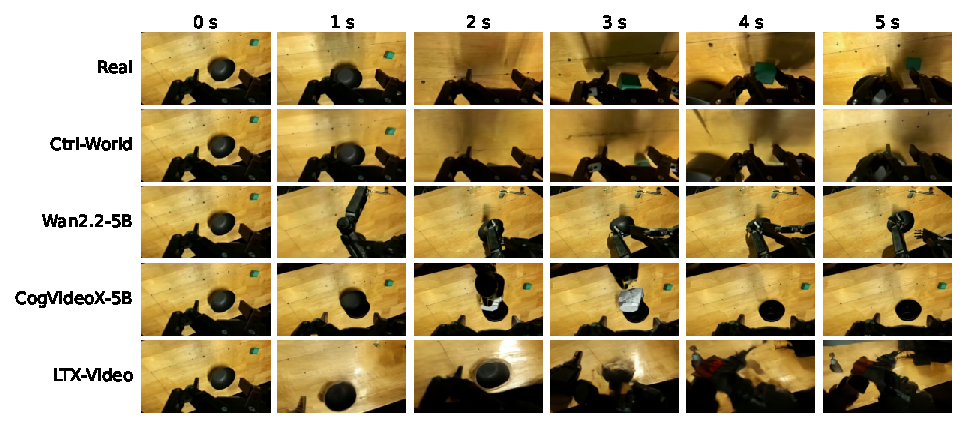
\includegraphics[width=\linewidth]{fig_qual_ep005.pdf}\\[4mm]
  \raggedright Ctrl-World follows the real camera motion but loses texture. Wan2.2 cuts to a
  third-person view, CogVideoX holds the view while objects morph, LTX distorts the scene.
}

\block{Scores on the 25 shared clips}{
  \centering\fontsize{30}{38}\selectfont\setlength{\tabcolsep}{8pt}
  \begin{tabular}{lcccc}
    \toprule
    & Motion (px) & Reg. $\uparrow$ & Fail $\downarrow$ & VGGT $\downarrow$ \\
    \midrule
    Real & 24.2 & 0.59 & 0.11 & 0.028 \\
    Slowed 2.5$\times$ & 10.9 & 0.66 & 0.060 & 0.013 \\
    Blurred & 23.7 & 0.76 & 0.15 & 0.029 \\
    Warp 8\,px & 24.6 & 0.70 & 0.15 & 0.045 \\
    Unrelated & 118.3 & 0.00 & 0.84 & 0.67 \\
    \midrule
    LTX & 10.3 & 0.25 & 0.32 & 0.024 \\
    CogVideoX & \hl{2.40} & 0.20 & 0.023 & \hl{0.007} \\
    Wan2.2 & \hl{2.57} & 0.27 & 0.043 & \hl{0.011} \\
    Ctrl-World & 19.7 & 0.26 & 0.36 & 0.031 \\
    \bottomrule
  \end{tabular}\\[4mm]
  \raggedright Near-static generators move about a tenth as much as reality and get the
  \emph{best} VGGT scores. Slowing real footage lowers VGGT disagreement too.
}

\block{Limitations}{
  One dataset and camera at low resolution; 25 shared clips; small open models; DROID-100 likely
  in Ctrl-World's training data; arm and object motion break rigidity; VGGT scores reflect its own
  predictions. We do not claim these scores predict planning success.
}

\column{0.5}
\block{1. Raw comparisons reward uninformative output}{
  Against the real continuation, a \textbf{frozen frame} has significantly lower match failure
  ($-$0.073), more inliers (+177) and lower VGGT disagreement ($-$0.031), while registering 64 points
  fewer frames. CogVideoX and Wan2.2 also look \emph{better} than real footage on their matchable clips.
}

\block{2. Motion-matched references shrink or remove the advantages}{
  \centering\fontsize{30}{38}\selectfont\setlength{\tabcolsep}{8pt}
  \begin{tabular}{llcccc}
    \toprule
    Model & vs. & Fail & VGGT & Reg. & $n$ \\
    \midrule
    CogVideoX & real & $-$0.26$^*$ & $-$0.039$^*$ & $-$0.29 & 6 \\
     & matched & $-$0.083$^*$ & \hl{$-$0.011$^*$} & $-$0.10 & 6 \\
    Wan2.2 & real & $-$0.18$^*$ & $-$0.010 & $-$0.20 & 6 \\
     & matched & $-$0.083 & \hl{+0.005} & $-$0.13 & 6 \\
    LTX & real & +0.32$^*$ & $-$0.000 & $-$0.41$^*$ & 15 \\
     & matched & +0.38$^*$ & +0.008 & $-$0.32$^*$ & 15 \\
    Ctrl-World & real & +0.23$^*$ & +0.000 & $-$0.39$^*$ & 22 \\
     & matched & +0.28$^*$ & \hl{+0.008$^*$} & $-$0.34$^*$ & 22 \\
    \midrule
    Frozen frame & real & $-$0.073$^*$ & $-$0.031$^*$ & $-$0.64$^*$ & 25 \\
    \bottomrule
  \end{tabular}\\[3mm]
  \raggedright{\fontsize{30}{38}\selectfont Model $-$ reference, 0.4\,s pairs. $^*$: 95\% CI excludes 0.}\\[4mm]
  CogVideoX's VGGT advantage shrinks by about 70\%; Wan2.2's disappears. The shift from raw to
  matched is significant for CogVideoX, Ctrl-World and LTX. Only 6--9 clips match for the
  near-static models, so per-model numbers are exploratory.
}

\block{3. Matching can also expose a hidden deficit}{
  Ctrl-World moves almost as much as reality (19.7 vs.\ 24.2\,px). Against the real continuation
  its VGGT disagreement shows no difference; against matched footage it is higher on the shared
  clips, though not significantly on all 60 clips. Registration is 33 points below real and
  50 below sharpness-matched blur, so blur does not explain it.
}

\block{A reporting protocol}{
  \innerblock{}{
    \begin{enumerate}
      \item Report image motion with two estimators (SIFT displacement, dense flow) and match coverage
      \item Always include a \textbf{frozen-frame} control
      \item Compare each clip against \textbf{motion- and appearance-matched real} footage
      \item Report the scores separately, never as one number
    \end{enumerate}
  }
  \vspace{4mm}
  A second scorer (StreamVGGT) agrees closely (Spearman $\rho=0.86$), but changes the raw LTX
  comparison, so raw scores can also depend on the scorer.
}

\block{A second clip}{
  \centering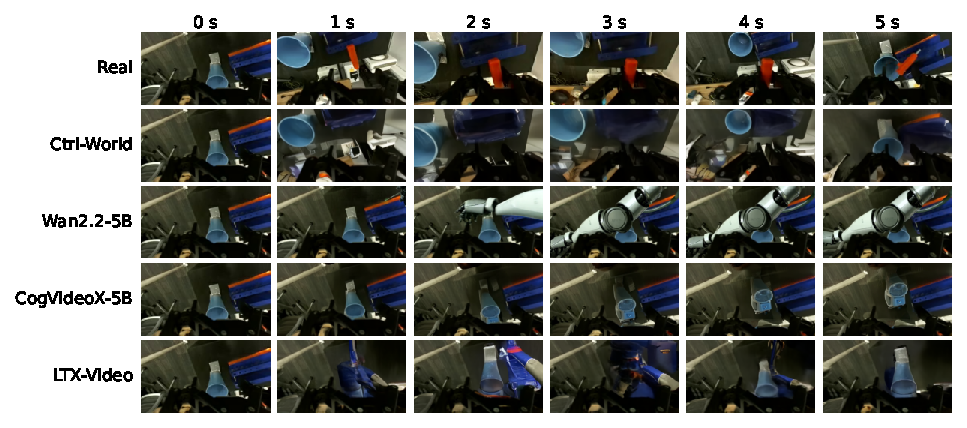
\includegraphics[width=\linewidth]{fig_qual_ep008.pdf}\\[4mm]
  \raggedright A clip near the median registration of Ctrl-World and LTX: Ctrl-World follows the
  camera's sweep; the others hold the view or distort it.
}

\end{columns}
\end{document}
